\chapter{Experimental result}
\label{Chap:4}
\section{Datasets}
\subsection{Market-1501}
\hspace{0.45cm} The Market-1501 dataset is collected in front of a super market in Tsinghua University. A total of six cameras were used, including 5 high-resolution cameras and one low-resolution camera.This dataset contains 32,668 annotated bounding boxes of 1501 indentities\cite{zheng2015scalable}. A visualization sample of dataset shown in fig.\ref{fig:market1501}
\begin{figure}[h!]
    \centering
    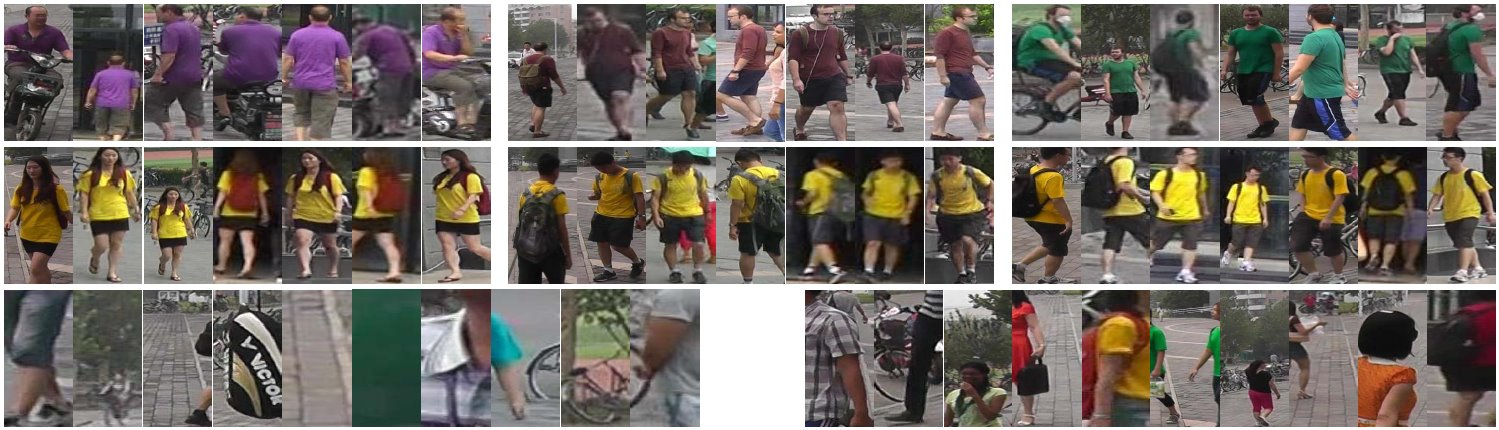
\includegraphics[width=0.6\textwidth]{Chapters/Fig/market-1501.jpg}
    \caption{Market-1501 dataset. The first two rows contain the image of training set while the third line contains the image of test set.}
    \label{fig:market1501}
\end{figure}
\subsection{MOT16}
\hspace{0.45cm} This dataset contains 14 sequences and are splitted into two half, ones for training and ones for testing. The annotations of the testing sequences will not be released in order to avoid over-fitting of the methods to the specific sequences \cite{Milan2016MOT16AB}.
Most sequences are filmed in high resolution, all images were converted to JPEG and named sequentially to a 6-digit file name (e.g. 000001.jpg). While detection and annotation files are simple comma-separated value (CSV) files.\par
Because, the ground truths of the test set were not provided, 
and the host of MOT challenge limits the time of each submit to evaluate results for the test set only once per 3 days. 
So, in this work, we would like to use only MOT16 train set which is not used to train any models in out work to evaluate the performance of the models.
\section{Experiments}
\subsection{Experimental environment}
\subsubsection{Hardware environment}
\hspace{0.45cm} All the models are running on a our local machine. The hardware specifications of which are listing in tab.\ref{tab:hardware_local}
\begin{table}[H]
\begin{center}
 \begin{tabular}{||c | c ||} 
 \hline
CPU & AMD Ryzen 5 1600 (6 cores, 16MB cache, 3.6GHz)\\
\hline
RAM & DDR4 8gb 3000MHz\\
\hline
GPU & GTX 1070 (8GB DDR5, 1920 cores, 1683Mhz) \\
\hline
Storage & HDD 1TB 7200rpm\\
 \hline
\end{tabular}
\end{center}
    \caption{Hardware specifications of local machine used in experiments}
    \label{tab:hardware_local}
\end{table}

% \begin{table}[H]
% \begin{center}
%  \begin{tabular}{||c | c ||} 
%  \hline
% CPU & 1xsingle core hyper threaded Xeon Processors @2.3Ghz\\
% \hline
% RAM & 12.6GB\\
% \hline
% GPU & 1xTesla K80 (2496 CUDA cores , 12GB GDDR5 VRAM) \\
% \hline
% Storage & 33GB\\
%  \hline
% \end{tabular}
% \end{center}
%     \caption{Hardware specifications of cloud machine used in experiments}
%     \label{tab:hardware_cloud}
% \end{table}

\subsubsection{Software}
\hspace{0.45cm}The following OS, libraries, tools, frameworks are utilized to implement our models:
\begin{itemize}
    \item \textbf{Ubuntu 16.04} a free and open-source Linux distribution
    \item \textbf{CUDA} is a revolutionary parallel computing architecture from NVIDIA\footnote{https://developer.nvidia.com}
    \item \textbf{cuDNN} or the NVIDIA CUDA Deep Neural Network library is the GPU-accelerated of primitives for deep neural network, 
    cuDNN provides highly tuned implementations for standard routined such as forward and backward convolution, pooling, normalization, 
    and activation layers.\footnote{https://developer.nvidia.com}
    \item \textbf{Anaconda} is a free and open-source distribution of the Python languages for scientific computing, that aims to simplify package management and deployment\footnote{Wikipedia}
    \item \textbf{Python 3.5} is version 3.5 of an interpreted, high-level, general purpose programming language
    \item \textbf{Pytorch 0.4} is a Python-based scientific computing package targeted in purpose of replacing NumPy to use the power of GPUs and to provide a deep learning research platform to maximize flexibility and speed\footnote{https://pytorch.org}
    \item \textbf{OpenCV 3.4.5} or Open Source Computer Vision Library is an open source computer vision and machine learning software library.\footnote{https://opencv.org}
\end{itemize}

\subsection{Implementation}

\subsubsection{SADeepSORT}
\hspace{0.45cm}Fortunately, the authors of \cite{Wojke2017simple} and \cite{SA} published their implementations for study purpose.
To have a fair comparison, we use these implementations in our experiments, moreover, we evaluate SADeepSORT on MOT16\cite{Milan2016MOT16AB} dataset using the same 
workflow of DeepSORT implementation which have the pre-generated detections using Faster \acrshort{RCNN} and deep appearance features for each frame in images sequence and 
that are compressed these data into a \textit{.npy} file corresponding to each sequence.
\cite{Wojke2017simple} is implemented using Python and TensorFlow for \acrshort{CNN} model to extract appearance feature.While \cite{SA} is implemented using Python and Pytorch, 
there is no pre-trained model because of limited connection to the mainland China website, we train the model on the Market-1501 dataset with pre-defined parameters and used the highest validation accuracy early stopping criteria.
We record the loss of training and the accuracy of validation during the training, the graph of validation accuracy is shown in fig.\ref{fig:val_acc_sa_train} while the graph of train loss is shown in fig.\ref{fig:loss_train_sa_train}.\par
\begin{figure}[h!]
    \centering
    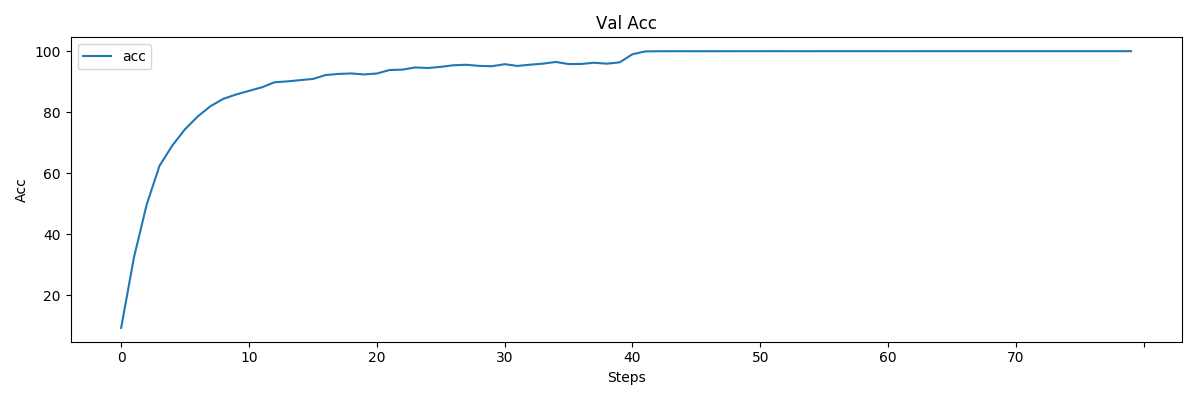
\includegraphics[width=0.7\textwidth]{Chapters/Fig/val_acc_sa_train.png}
    \caption{Accuracy of validation during training process Parameter-free Spatial Network}
    \label{fig:val_acc_sa_train}
\end{figure}
\begin{figure}[h!]
    \centering
    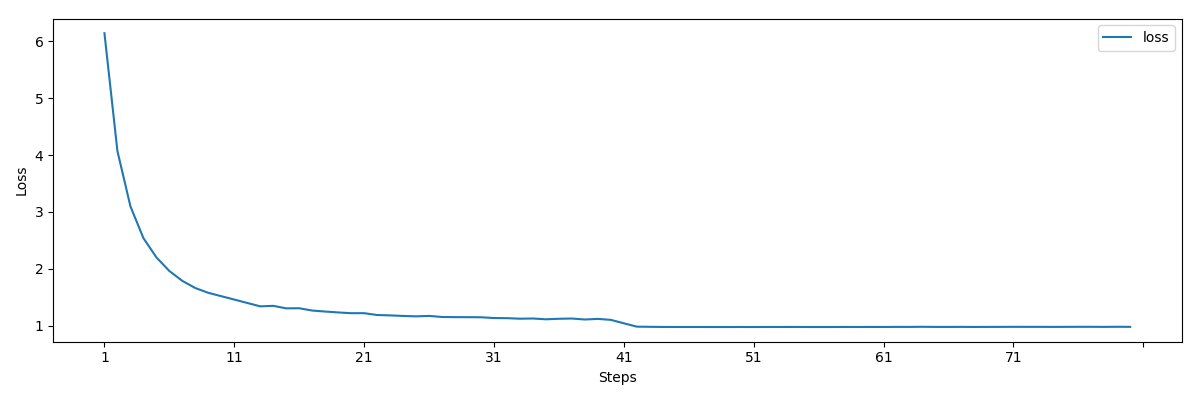
\includegraphics[width=0.7\textwidth]{Chapters/Fig/loss_train_sa.png}
    \caption{Training loss during training process Parameter-free Spatial Network}
    \label{fig:loss_train_sa_train}
\end{figure}
Then, we compress the data of detections by Faster \acrshort{RCNN}\cite{Wojke2017simple} and appearance features by Spatial Attention Network into \textit{.npy} files for each sequence
Finally, we use these \textit{.npy} files with tracking and associating implementation part of DeepSORT\cite{Wojke2017simple} to perform the experiment on MOT16 dataset.
.\par
\subsubsection{YOLOv3-DeepSORT}
\hspace{0.45cm}Original version of YOLOv3 was implemented in C++ which we are not familiar with. However, the authors of \cite{yolov3} provided a \textit{cfg} (e.g. config) file which contain list of layer's name and pre-defined hyperparameter 
such as filters number, stride, padding or activation function name.\par For example, a convolutional layer defined in \textit{cfg} file:
\begin{lstlisting}
    [convolutional]
    batch_normalize=1
    filters=32
    size=3
    stride=1
    pad=1
    activation=leaky
\end{lstlisting}\par
We parse this \textit{cfg} file to a list and build a Pytorch version of YOLOv3 using this list. We load the weights to the network using \textit{weight} file which is also provided by the authors of \cite{yolov3},
 the weights were obtained by training YOLOv3 on COCO2014 dataset. Then we filter the output of our Pytorch-YOLOv3 so that now only returns detections with person class label.\par
% Because the original CNN model to extract appearance was implemented in TensorFlow which we are not familiar with, so we re-implemented it in Pytorch and train it Mars dataset as same as the original version.\par
We use our Pytorch-YOLOv3 and use the CNN, tracking and associating implementations of DeepSORT\cite{Wojke2017simple} to perform experiment on MOT16 dataset.

\subsection{Experimental Results}
\hspace{0.45cm}To evaluate the result using metrics mentions in section, we use a Python tool suggested by the host of MOT challenge\footnote{https://motchallenge.net}, which is \textit{py-motmetrics}\footnote{https://github.com/cheind/py-motmetrics}.
Evaluation measures with ($\uparrow$), higher scores denote better performance, while evaluation measures with ($\downarrow$), lower scores denote better performance \cite{sort}, the details of evaluation metrics mentioned in previous chapter.\par
\subsubsection{SADeepSORT}
\hspace{0.45cm}We have two tables that represent performance on MOT16 dataset which are evaluated using \textit{py-motmetrics}\footnote{https://github.com/cheind/py-motmetrics} tool and the speed of SADeepSORT and DeepSORT\cite{Wojke2017simple}. 
% \begin{table}[H]
% \begin{center}
%  \begin{tabular}{||c | c | c | c | c | c | c | c | c ||} 
%  \hline
% Sequence & GT & MT($\uparrow$)  & ML($\downarrow$) & FP($\downarrow$) & FN($\downarrow$) & IDs($\downarrow$) & MOTA($\uparrow$) & MOTP($\uparrow$) \\
% \hline
% \hline
% MOT16-02 & 54 & 7 &  19 & 1238 & 11048 & 53 & 30.8\% & 0.178 \\
%  \hline
% MOT16-04 & 83 & 35 &  18 & 4336 & 16011 & 49 & 57.1\% & 0.160\\
% \hline
% MOT16-05 & 125 & 18 &  35 & 235 & 3036 & 35 & 51.5\% & 0.206 \\
% \hline
% MOT16-09 & 25 & 11 &   2 & 116 & 1879 & 18 & 61.7\% & 0.152 \\
% \hline
% MOT16-10 & 54 & 15 &   8 & 1016 & 4590 & 69 & 53.9\% & 0.212 \\
% \hline
% MOT16-11 &  69 &  15  & 23 & 195 & 3135 & 18 & 63.5\% & 0.134\\
% \hline
% MOT16-13 & 107 & 29  & 27 & 280 & 4589 & 70 & 56.9\% & 0.212\\
% \hline
% OVERALL  & 517 & 130  & 132 & 7416 & 44288 & 312 & 52.9\% & 0.173\\

% \hline
% \end{tabular}
% \end{center}
%     \caption{Results on MOT16 train set using original DeepSORT model}
%     \label{tab:org_result}
% \end{table}
% \begin{table}[H]
%     \begin{center}
%      \begin{tabular}{||c | c | c | c | c | c | c | c | c | c ||} 
%      \hline
%     Sequence & GT & MT($\uparrow$) & ML($\downarrow$) & FP($\downarrow$) & FN($\downarrow$) & IDs($\downarrow$) & MOTA($\uparrow$) & MOTP($\uparrow$) \\
%     \hline
%     \hline
%     MOT16-02 & 54 &  8  & 20 & 1228 & 11086 & 49 & 30.7\% & 0.178 \\
%      \hline
%     MOT16-04 & 83 & 35  & 18 & 4346 & 15996 &  41 & 57.1\% & 0.160\\
%     \hline
%     MOT16-05 & 125 & 19  & 35 & 247 & 3014 & 30 & 51.7\% & 0.205 \\
%     \hline
%     MOT16-09 & 25 & 12  &  2 & 116 & 1870 & 17 & 61.9\% & 0.151 \\
%     \hline
%     MOT16-10 & 54 & 14  & 8 & 1025 & 4593 & 66 & 53.9\% & 0.213 \\
%     \hline
%     MOT16-11 &  69 &  15 &  22 & 189 & 3116 & 17 & 63.8\% & 0.134\\
%     \hline
%     MOT16-13 & 107 & 30 &  26 & 278 & 4554 & 68 & 57.2\% & 0.212\\
%     \hline
%     OVERALL  & 517 & 133 &  131 & 7429 & 44229 & 288 & 53.0\% & 0.17\\
    
%     \hline
%     \end{tabular}
%     \end{center}
%         \caption{Results on MOT16 train set using SADeepSORT}
%         \label{tab:sa_result}
% \end{table}
\pagebreak

\begin{landscape}
\begin{table}[H]
    \centering
    \begin{tabular}{||c|c|c|c|c|c|c|c|c|c|c|c|c|c|c|c||}
        \hline
        \multirow{2}{*}{Sequence} & \multirow{2}{*}{GT} & \multicolumn{2}{c|}{MT($\uparrow$)} & \multicolumn{2}{c|}{ML($\downarrow$)} & \multicolumn{2}{c|}{FP($\downarrow$)} & \multicolumn{2}{c|}{FN($\downarrow$)} & \multicolumn{2}{c|}{IDs($\downarrow$)} & \multicolumn{2}{c|}{MOTA($\uparrow$)} & \multicolumn{2}{c|}{MOTP($\uparrow$)} \\ \cline{3-16} 
                 &     & I   &  II                   &   I & II                    &  I   &  II                    &  I            &  II                     & I   & II                   &  I     &    II                     &    I  &    II       \\ \hline
        MOT16-02 & 54  & 7   & \textcolor{blue}{8}   & 19  & \textcolor{red}{20}   & 1238 & \textcolor{blue}{1228} &  11048        & \textcolor{red}{11086}  & 53  & \textcolor{blue}{49} & 30.8\% & \textcolor{red}{30.7}\%   & 0.178 & 0.178          \\ \hline
        MOT16-04 & 83  & 35  & 35                    & 18  & 18                    & 4336 & \textcolor{red}{4346}  &  16011        & \textcolor{blue}{15996} & 49  & \textcolor{blue}{41} & 57.1\% & 57.1\%                    & 0.160 & 0.160         \\ \hline
        MOT16-05 & 125 & 18  & \textcolor{blue}{19}  & 35  & 35                    & 235  & \textcolor{red}{247}   &  3036         & \textcolor{blue}{3014}  & 35  & \textcolor{blue}{30} & 51.5\% & \textcolor{blue}{51.7}\%  & 0.206 & \textcolor{red}{0.205}          \\ \hline
        MOT16-09 & 25  & 11  & \textcolor{blue}{12}  & 2   & 2                     & 116  & 116                    &  1879         & \textcolor{blue}{1870}  & 18  & \textcolor{blue}{17} & 61.7\% & \textcolor{blue}{51.9}\%  & 0.152 & \textcolor{red}{0.151}          \\ \hline
        MOT16-10 & 54  & 15  & \textcolor{red}{14}   & 8   & 8                     & 1016 & \textcolor{red}{1025}  &  4590         & \textcolor{red}{4593}   & 69  & \textcolor{blue}{66} & 53.9\% & 53.9\%                    & 0.212 & \textcolor{blue}{0.213}          \\ \hline
        MOT16-11 & 69  & 15  & 15                    & 23  & \textcolor{blue}{22}  & 195  & \textcolor{blue}{189}  &  3135         & \textcolor{blue}{3116}  & 18  & \textcolor{blue}{17} & 63.5\% & \textcolor{blue}{63.8}\%  & 0.134 & 0.134          \\ \hline
        MOT16-13 & 107 & 29  & \textcolor{blue}{30}  & 27  & \textcolor{blue}{26}  & 280  & \textcolor{blue}{178}  &  4589         & \textcolor{blue}{4554}  & 70  & \textcolor{blue}{68} & 56.9\% & \textcolor{blue}{57.2}\%  & 0.212 & 0.212          \\ \hline
        OVERALL  & 517 & 130 & \textcolor{blue}{133} & 132 & \textcolor{blue}{131} & 7416 & \textcolor{red}{7429}  &  44288        & \textcolor{blue}{44229} & 312 & \textcolor{blue}{288} & 52.9\% & \textcolor{blue}{53.0}\% & 0.173 & \textcolor{red}{0.17}          \\ \hline
    \end{tabular}
    \caption{Results on MOT16 dataset of DeepSORT(I) and SADeepSORT(II) evaluated by \textit{py-motmetrics}. Value with red color is worse while the blue one is better}
    \label{tab:sa_deepsort_result}
\end{table}
\end{landscape}

\pagebreak



\begin{table}[H]
    \begin{center}
     \begin{tabular}{||c | c | c ||} 
     \hline
    Sequence & SADeepSORT (\acrshort{FPS}) & DeepSORT\cite{Wojke2017simple} (\acrshort{FPS}) \\
    \hline
    \hline
    MOT16-02 & 8 & 20 \\
     \hline
    MOT16-04 & 4 & 16.4\\
    \hline
    MOT16-05 & 20.5 & 47 \\
    \hline
    MOT16-09 & 15.4 & 25.7 \\
    \hline
    MOT16-10 & 9.2 & 20.7\\
    \hline
    MOT16-11 &  15.3 &  25.3\\
    \hline
    MOT16-13 & 10.6 & 22.7\\
    \hline
    AVERAGE  & 11.8 & 25.4 \\
    
    \hline
    \end{tabular}
    \end{center}
        \caption{\acrshort{FPS} on MOT16 dataset\cite{Milan2016MOT16AB} of SADeepSORT and DeepSORT\cite{Wojke2017simple}}
        \label{tab:fps_com}
\end{table}

According tab.\ref{tab:sa_deepsort_result} and tab.\ref{tab:fps_com}, SADeepSORT is slightly better overall results than DeepSORT\cite{Wojke2017simple}
. Concretely, SADeepSORT has less overall \acrshort{FN},\acrshort{FP} and \acrshort{IDs} which leads to better \acrshort{MOTA} than DeepSORT\cite{Wojke2017simple}, moreover, 
SADeepSORT provides more \acrshort{MT} tracks than DeepSORT\cite{Wojke2017simple}. However, the computational time of SADeepSORT is much slower than DeepSORT\cite{Wojke2017simple}.



\subsubsection{YOLOv3-DeepSORT}

\hspace{0.45cm}MOT metrics\cite{Milan2016MOT16AB} evaluates the performance of a tracker based on evaluating the hypothesis and the ground truth with respect to the \textbf{ID}, it means that
when our \textbf{ID} of our hypothesis is \textit{1}, it will be used to compute evaluation metrics with the ground truth with \textbf{ID} \textit{1}. However, the detection results obtained
by our YOLOv3 is not mapped with the annotations of the dataset. Therefore, using MOT metrics \cite{Milan2016MOT16AB} is not reliable in this case.\par 

\begin{table}[H]
\begin{center}
    \begin{tabular}{|| c | c | c ||} 
    \hline
    & YOLOv3\cite{yolov3} & Faster \acrshort{RCNN} \cite{Wojke2017simple}  \\
    \hline
    \hline
    MOT16-02 & 9048 & 14092\\
    \hline
    MOT16-04 & 32347 & 40790\\
    \hline
    MOT16-05 & 9813 & 5115 \\
    \hline
    MOT16-09 & 6328 & 4218 \\
    \hline
    MOT16-10 & 10095 & 13208\\
    \hline
    MOT16-11 & 11523 & 8394\\
    \hline
    MOT16-13 & 6205 & 13818\\
    \hline
    Overall & 85354 & 99635 \\
    \hline

\end{tabular}
\end{center}
    \caption{Person detection results of YOLOv3\cite{yolov3} versus Faster \acrshort{RCNN}}
    \label{tab:detections_results}
\end{table}

YOLOv3 pretrained on COCO 2014 dataset is able to detect 80 different class labels \cite{yolov3}, it means that YOLOv3 is not optimized to detect only person class label. Consequently, 
we found out that, the overall number of person detections of the YOLOv3\cite{yolov3} model we implemented is much smaller than the Faster \acrshort{RCNN} detector of \cite{Wojke2017simple}. Moreover, 
in tracking-by-detection framework, the performance of the detection algorithms is the proportional key factor to the performance of the tracking system. Therefore,
we can assume that replacing Faster \acrshort{RCNN} with YOLOv3\cite{yolov3} leads to poor overall performance.

\begin{figure}[h!]
    \centering
    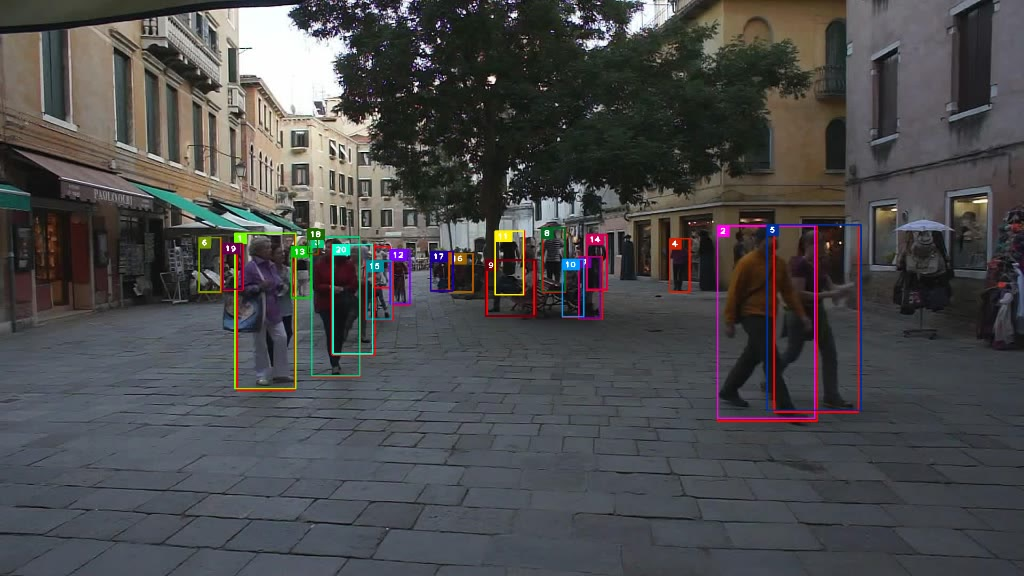
\includegraphics[width=\textwidth]{Chapters/Fig/mot02_org_1.jpg}
    \caption{Visualization of detections and tracks in MOT16-02 sequence obtained by DeepSORT\cite{Wojke2017simple}}
    \label{fig:mot02_org_1}
\end{figure}

\begin{figure}[h!]
    \centering
    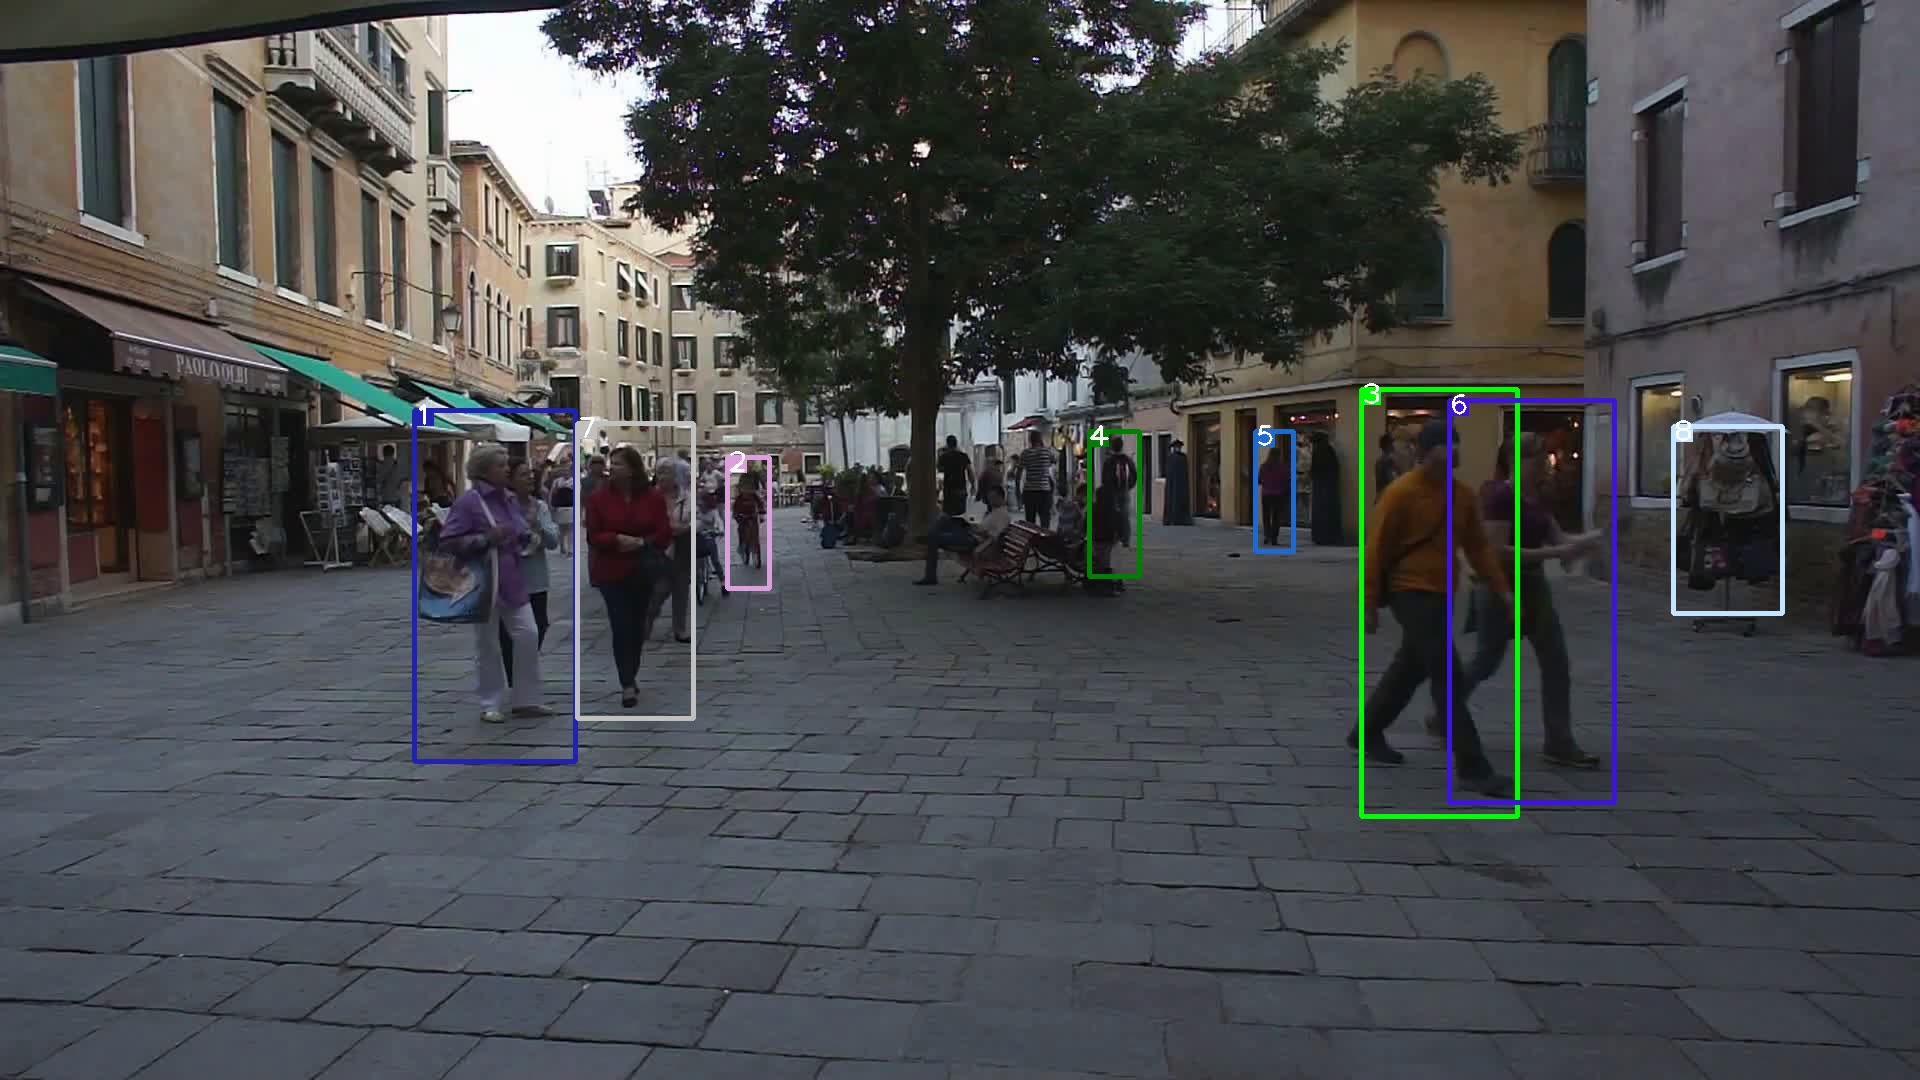
\includegraphics[width=\textwidth]{Chapters/Fig/mot02_yolo_1.jpg}
    \caption{Visualization of detections and tracks in MOT16-02 sequence obtained by YOLOv3-DeepSORT}
    \label{fig:mot02_yolo_1}
\end{figure}

According to the tab.\ref{tab:detections_results}, in MOT16-02 sequence, YOLOv3\cite{yolov3} provided a smaller number of detections than
Faster \acrshort{RCNN} in \cite{Wojke2017simple}, and the visualizations of detections in MOT16-02 sequence of two detection algorithms are shown in
fig.\ref{fig:mot02_org_1} and fig.\ref{fig:mot02_yolo_1}. In this sequence, people perform different poses such as
sitting, walking, riding; the color of the clothes are close to the color of the background and the scale of individual person is small.
These reasons may lead the the poor result of YOLOv3\cite{yolov3} in person detection.
\begin{figure}[h!]
    \centering
    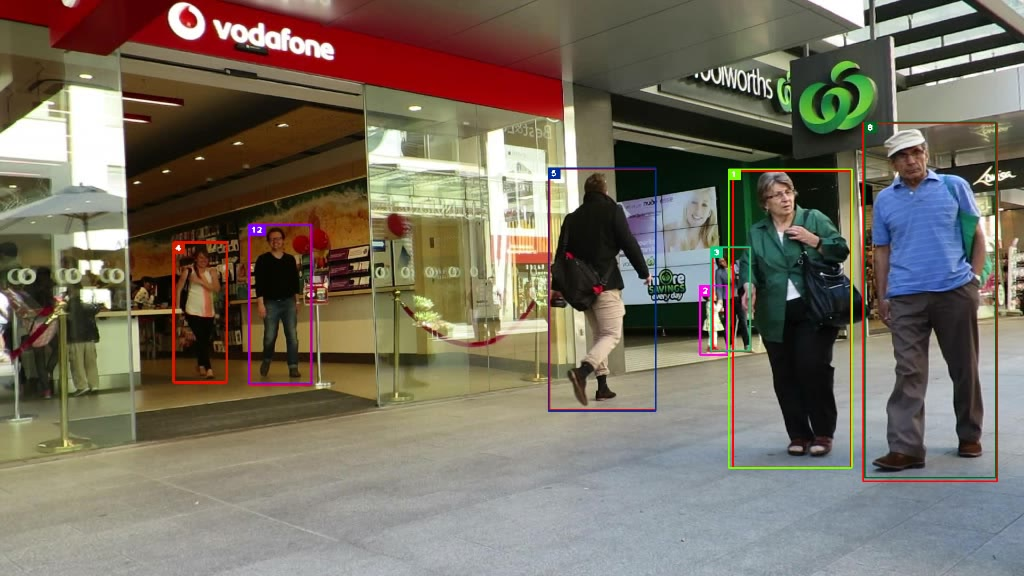
\includegraphics[width=\textwidth]{Chapters/Fig/mot09_org_1.jpg}
    \caption{Visualization of detections and tracks in MOT16-09 sequence at frame $\text{97}^{th}$ obtained by Faster \acrshort{RCNN} in DeepSORT\cite{Wojke2017simple}}
    \label{fig:mot09_org_1}
\end{figure}

\begin{figure}[h!]
    \centering
    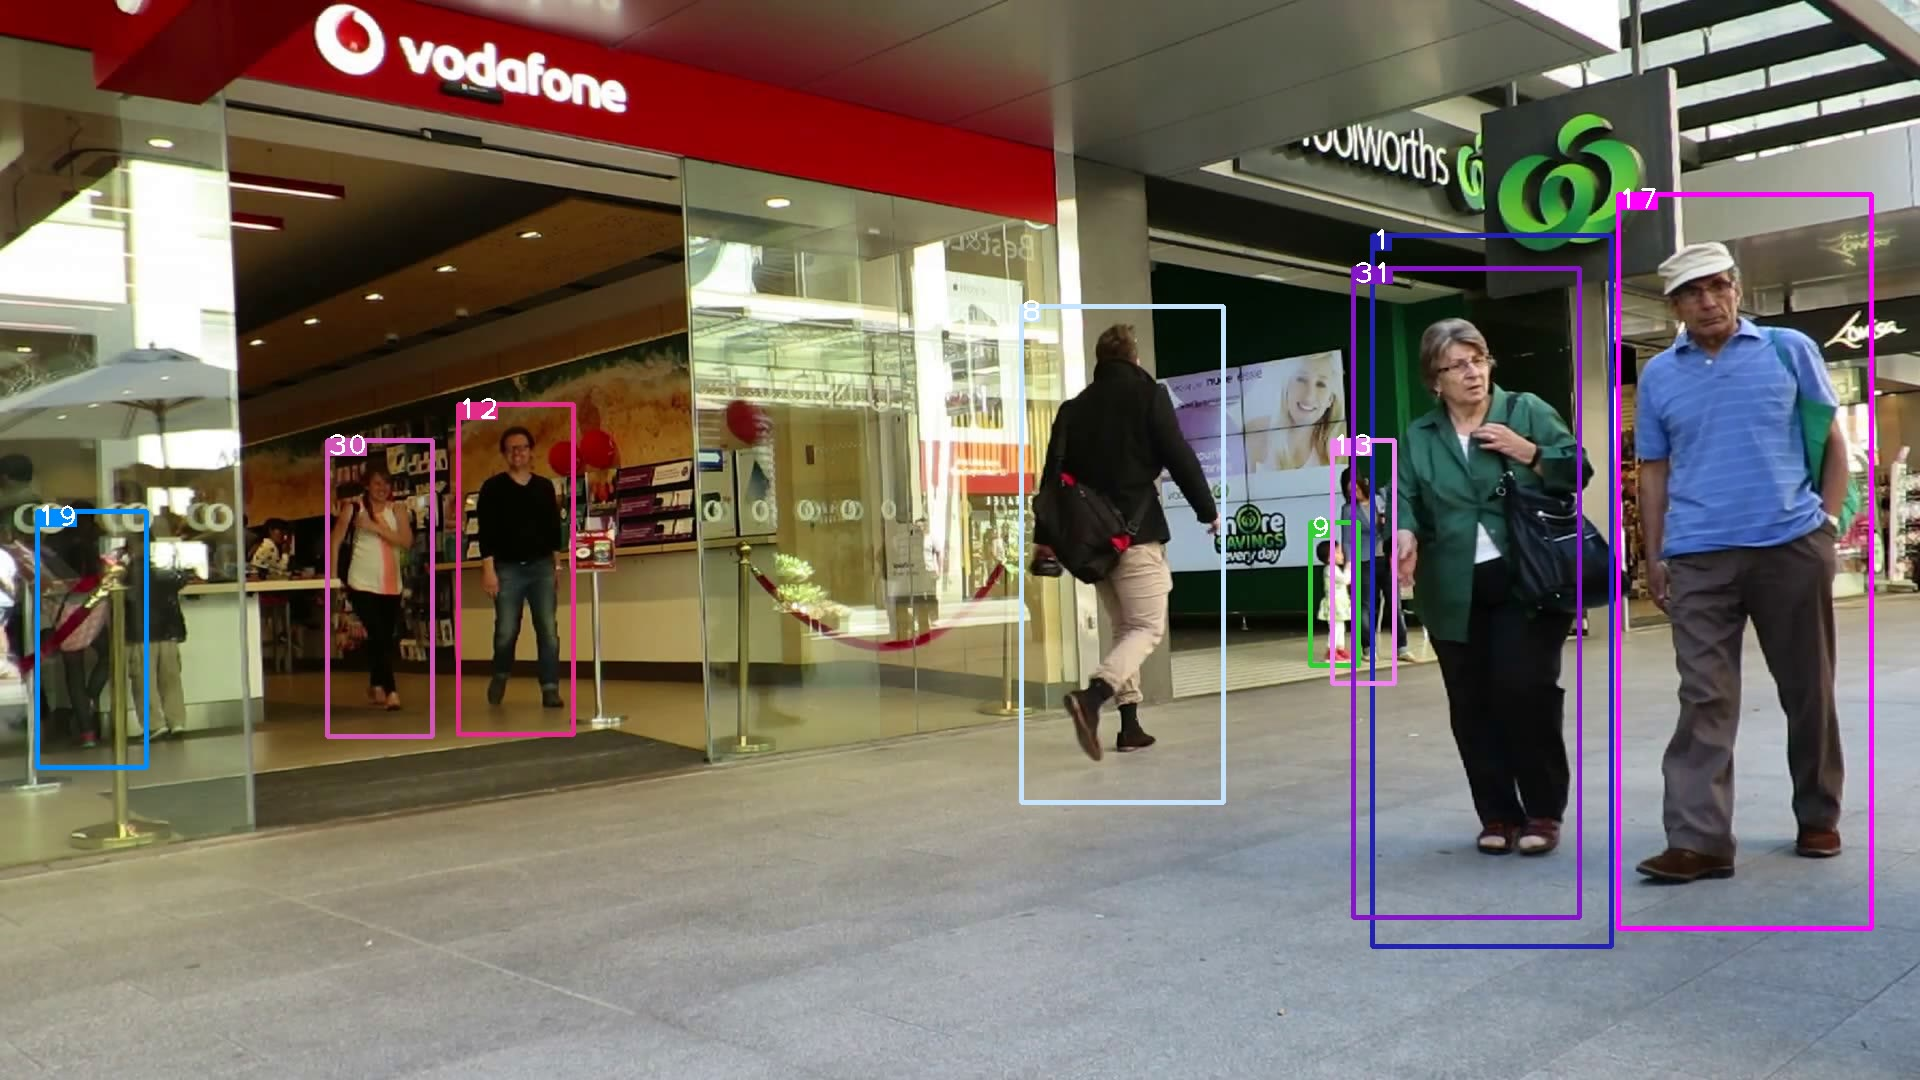
\includegraphics[width=\textwidth]{Chapters/Fig/mot09_yolo_1.jpg}
    \caption{Visualization of detections and tracks in MOT16-09 sequence at frame $\text{97}^{th}$ obtained by YOLOv3}
    \label{fig:mot09_yolo_1}
\end{figure}
\pagebreak
\begin{figure}[h!]
    \centering
    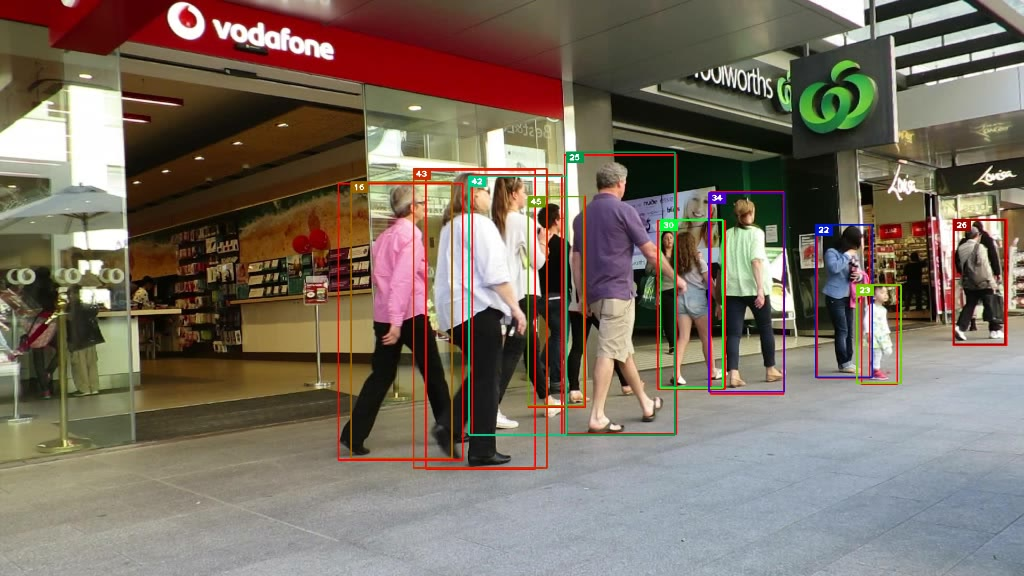
\includegraphics[width=\textwidth]{Chapters/Fig/mot09_org_2.jpg}
    \caption{Visualization of detections and tracks in MOT16-09 sequence at frame$\text{252}^{nd}$ obtained by Faster \acrshort{RCNN} in DeepSORT\cite{Wojke2017simple}}
    \label{fig:mot09_org_2}
\end{figure}

\begin{figure}[h!]
    \centering
    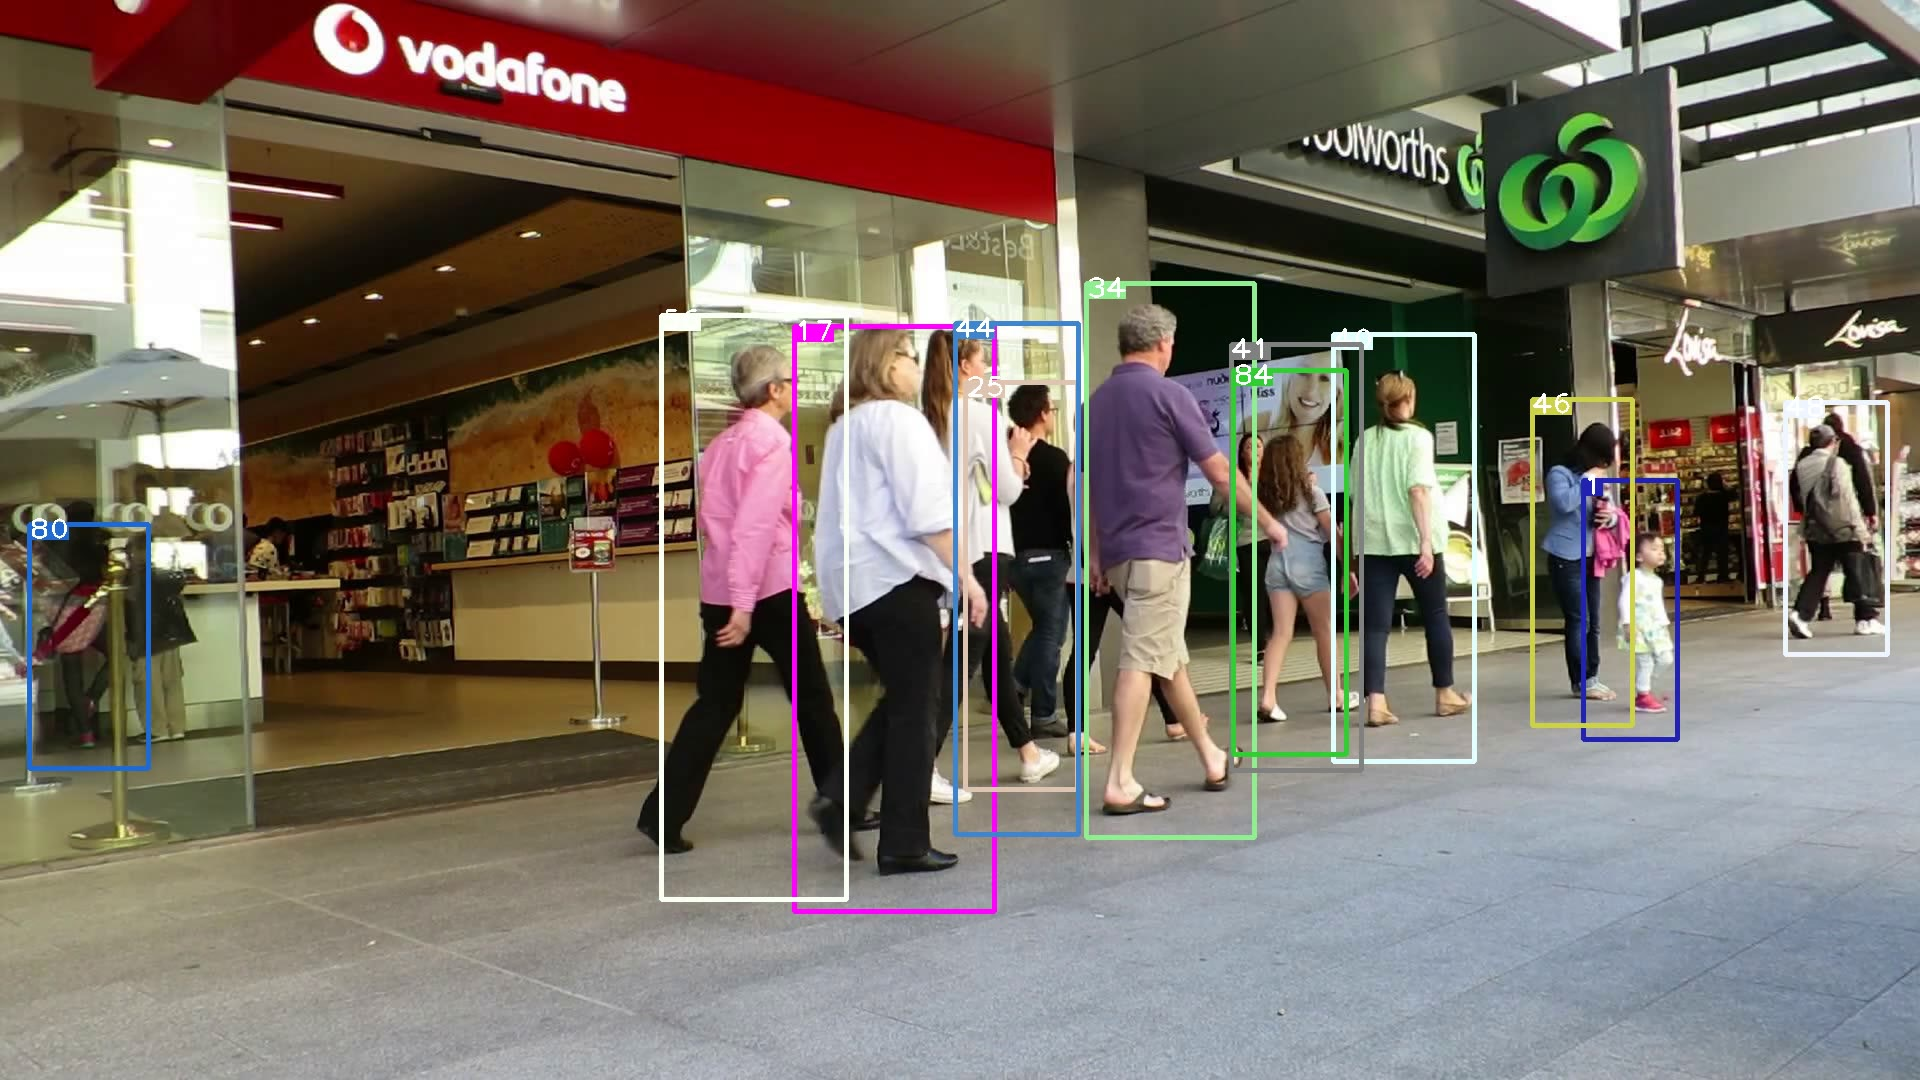
\includegraphics[width=\textwidth]{Chapters/Fig/mot09_yolo_2.jpg}
    \caption{Visualization of detections and tracks in MOT16-09 sequence at frame $\text{252}^{nd}$ obtained by YOLOv3}
    \label{fig:mot09_yolo_2}
\end{figure}\par
However, in the MOT16-09 sequence, YOLOv3\cite{yolov3} provided a larger number
of person detections than Faster \acrshort{RCNN} in \cite{Wojke2017simple}, we visualize the detections of two detection algorithms in fig.\ref{fig:mot09_org_1},
fig.\ref{fig:mot09_yolo_1}, fig.\ref{fig:mot09_org_2} and fig.\ref{fig:mot09_yolo_2}. In this sequence, mostly people are walking; 
the light of the background is lighter than MOT16-02, so the color of the clothes is more easier to distinguish than in MOT16-02. These may 
lead YOLOv3 \cite{yolov3} does better detects person than Faster \acrshort{RCNN} in \cite{Wojke2017simple}.We can also behold that YOLOv3\cite{yolov3}
can detect a person who stands behind the glass with complex lights (reflections) on it while Faster \acrshort{RCNN} in \cite{Wojke2017simple}
is not able to do it. Hypothesis target with id \textit{19} the fig.\ref{fig:mot09_yolo_1} is not appeared in the fig.\ref{fig:mot09_org_1},
hypothesis target with id \textit{80} the fig.\ref{fig:mot09_yolo_2} is not appeared in the fig.\ref{fig:mot09_org_2},


\chapter{Conclusions and Future Work}
\hspace{0.45cm} This chapter consists the thesis contributions, limitations and discuss further development from the proposals presented in above chapters.
\section{Conclusions}
\hspace{0.45cm} In this thesis, we propose two alterations in the architecture of DeepSORT\cite{Wojke2017simple}, a online and real time pedestrian trackings that achieved competitive results in MOT challenges. Then, we create experiments to evaluate the performance of two proposals and compare these results with DeepSORT.\par
The first proposal in the thesis is using Parameter-free Spatial Attention network for person re-identification \cite{SA} to extract deep appearance features instead of using a simply CNN architecture as \cite{Wojke2017simple}. The first proposal has a better results but the improvement is not so noticeable while speed to much slower.\par
The second proposal in the thesis is replacing Faster \acrshort{RCNN} with YOLOv3 as the main detector in the DeepSORT \cite{Wojke2017simple}. Because the mapping IDs between the hypothesis ID and the ground truth ID is not done yet so the results obtained from MOT metrics is not reliable. We consider number of the detections of YOLOv3 pretrained on COCO 2014 dataset by \cite{yolov3} which is then modified to select only person class label detections  and the Faster \acrshort{RCNN} pretrained on several datasets \cite{Wojke2017simple}.
Because the quality of detector influences proportionally on the performance of tracking methods and the overall person detection of YOLOv3\cite{yolov3}
is much smaller than Faster \acrshort{RCNN} of DeepSORT\cite{Wojke2017simple}, then we can say that YOLOv3-DeepSORT perform worse than DeepSORT\cite{Wojke2017simple}
on MOT16 dataset.

\section{Thesis contributions}
The contribution of this thesis consists numerous aspects listed below:
\begin{itemize}
    \item The detail explanation of architecture, workflows of DeepSORT\cite{Wojke2017simple} - a online and realtime pedestrian tracking
     using recent advancement in deep learning and its related backgrounds.
    \item The proposals of architecture and workflow alterations in order to increase the performance of the DeepSORT\cite{Wojke2017simple}
    \item The detailed results comparisons and analyses between our two proposals and DeepSORT\cite{Wojke2017simple} using both MOT metrics\cite{Milan2016MOT16AB} and visualizations
\end{itemize}
\section{Limitations}
\hspace{0.45cm}There are some limitations in our experiments that make our proposals are unable to perform better than DeepSORT\cite{Wojke2017simple}
on MOT16 dataset:
\begin{itemize}
    \item \acrshort{SA} network used to extract deep appearance features that was trained on Market-1501 dataset has ResNet-50\cite{He_2016_CVPR} backbone. 
    ResNet-50\cite{He_2016_CVPR} is a very deep network or in the other work, computational cost of ResNet-50\cite{He_2016_CVPR} is expensive which may limit the real time constraint of the system.
    \item YOLOv3 provided by Joseph et at.\cite{yolov3} was trained on COCO 2014 which has 80 class labels and not optimized for only person detecting. Consequently, person who is not standing or walking in the scene may be not detected in our experiment.
    \item YOLOv3 detection results are not mapped with annotations that lead to using MOT metrics\cite{Milan2016MOT16AB} is not reliable
    to evaluate performance of YOLOv3-DeepSORT on MOT16 dataset.
\end{itemize}

\section{Future Work} 
\hspace{0.45cm} The results in our first experiment of SADeepSORT is not so significant better than DeepSORT\cite{Wojke2017simple} while
the speed is slower due to the limitation we mentions in previous section. We want to train the parameter-free spatial attention
network with different backbone architectures which should be shallower than ResNet-50\cite{He_2016_CVPR} but still remain the competitive results.
With these experiments, we expect to have a online pedestrian tracking method that achieve real-time constraint and asymptotically state-of-the-art result.\par 
The YOLOv3\cite{yolov3} that is pretrained on COCO 2014 dataset used in our second experiment did not perform well in person detection 
when compares with Faster \acrshort{RCNN} in \cite{Wojke2017simple}. We want to modify some hyperparameter of YOLOv3 such as the predefined dimensions of
anchor box to make it robust to the size of person which different poses and then train it on person detection dataset. After that,
we expect to acquire a more accurate and faster person detector than original YOLOv3\cite{yolov3} and Faster \acrshort{RCNN} in \cite{Wojke2017simple}.\par 
Then we are going the determine a mapping of the detection results of different detector to the annotated detections to make
MOT metrics\cite{Milan2016MOT16AB} to be more reliable to allow us to attend in the upcoming challenges of MOT challenge\footnote{https://motchallenge.net}.\par
Finally, we aim to implement the tracking algorithm in a more power programming language like C/C++ to maximize the speed and apply the algorithm
on surveillance system in a restaurants, stores or offices.